% TP1 - Algorithmic Music Composition (UFMG)
% Official ISMIR 2026 template (https://github.com/ismir/paper_templates, 2026/latex).
% Limit for graduate students: 3 pages of content. References, AI Usage Statement and
% Acknowledgments do not count.
\documentclass{article}
\usepackage[T1]{fontenc}
\usepackage[utf8]{inputenc}
% Without the "submission" option the author name is shown and line numbers are off.
% Note: in this mode ismir.sty prints "in Proc. of the 27th Int. Society for Music
% Information Retrieval Conf." in the first-page footnote. Ask the professor if that is ok.
\usepackage{ismir}
\usepackage{amsmath,cite,url}
\usepackage{graphicx}
\usepackage{color}
\usepackage{booktabs}

\title{A Genetic Algorithm for Jazz Tenor Saxophone Melodies over a ii-V-I Progression}

\oneauthor
  {Carlos Le\~{a}o}
  {Universidade Federal de Minas Gerais (UFMG)\\\texttt{your.email@ufmg.br}}

% Used in the copyright notice: abbreviated first name.
\def\authorname{C. Le\~{a}o}

\sloppy

\begin{document}

\maketitle

\begin{abstract}
% About 150 words. One or two sentences each:
% - problem: symbolic melody generation with a genetic algorithm
% - style constraint: jazz tenor sax, ii-V-I loop in C major (Dm7 | G7 | Cmaj7 | Cmaj7), 12 bars
% - method: eighth-note genome, rule-based fitness with 5 rules from jazz theory and the
%   Weimar Jazz Database
% - experiment: mutation rate 0.01, 0.05, 0.2 with 3 seeds each
% - main result: 0.01 reaches the highest fitness; 0.2 stalls

\end{abstract}

\section{Introduction}\label{sec:introduction}
% About 1/3 of a column.
% - Motivation: why generate jazz melodies, why a GA (fitness can encode music theory,
%   every rule is explainable).
% - Style constraint (mandatory to state): jazz tenor sax solo over a fixed ii-V-I loop in
%   C major, 12 bars, 170 BPM, swing applied at playback.
% - What the system outputs: MIDI, rendered to WAV with FluidSynth.
% - Contributions in one or two sentences, and where the code and audio are
%   (\url{https://github.com/Chbmleao/jazz-sax-ga}).
TODO

\section{Related Work}\label{sec:related}

Horner and Goldberg \cite{horner1991} published the first use of a genetic algorithm (GA) for music composition. Since then, several directions of GA application to melody composition have emerged. One notable example is GenJam \cite{biles1997}, which uses an interactive genetic algorithm, in other words, a human-in-the-loop fitness evaluation. The system evolves two populations of musical elements (measures and phrases), with notes mapped to the scale of the current chord. The fitness of each individual comes from a human mentor, who gives real-time feedback by typing ``g'' for good or ``b'' for bad. This approach exposes the ``fitness bottleneck'': human evaluation limits the speed and scalability of the evolutionary process. In contrast, our work replaces the human mentor with jazz theory rules, so the fitness is evaluated automatically.

Besides interactive approaches, another line of research computes the fitness automatically from general music theory rules. Ozcan and Ercal \cite{ozcan2008} present AMUSE, a GA-based system that generates improvised melodies over a given harmonic context. Each gene is a scale degree, where 0 is a rest and the maximum value is a hold. Its fitness function combines ten objectives based on music theory, including rules for chord tones, relationships between notes, directions of notes, the beginning and ending notes of the melody, and the proportion of rests. In a Turing test, listeners had to tell apart solos generated by the GA from solos written by an amateur musician, and 52\% of them gave the wrong answer, which suggests that the generated solos are comparable to an amateur's. Our work builds on this approach, using a similar rest/hold encoding and a fitness that combines several objectives.

Mati\'c \cite{matic2010} also uses an automatic fitness, to compose short melodies of four bars. The genome follows the same rest/hold encoding, with one integer per eighth note, where 0 is a rest, the values from 1 to $n$ are pitches relative to a reference note, and $n+1$ is a hold. The fitness is minimized and computed bar by bar as a weighted sum of the quality of each interval, the mean and variance of the intervals compared with reference values, and a penalty for notes outside the key. Since the melodies are short, the GA uses no crossover, only three mutations: moving a note by an octave, changing one note, and swapping two neighboring notes. The author reports that the GA tends to produce many rests, because rests avoid bad intervals. In contrast, our work keeps crossover, at bar lines, and rests come from an explicit breathing rule instead of being a side effect of avoiding bad intervals.

Besides these general techniques, Wiggins et al. \cite{wiggins1998} argue that the results of a GA depend heavily on the domain-specific knowledge in its operators and fitness function. Their jazz solo generator represents a solo as a list of (scale degree, duration) genes over a chord progression, and its fitness checks eight features, such as illegal jumps, long notes, speed, and pattern matching. They found that too much weight on pattern matching led to repetitive and boring solos. They also note that their systems have neither a clear plan nor intention, and that large-scale structure cannot be expected from a GA with little domain knowledge, a limitation that our work shares.

\section{Methodology}\label{sec:methodology}
% The assignment requires all of: genotype, initial population, fitness (with a justification
% for each rule), selection, crossover, mutation and stopping criterion.
% About 1 column. Details are in docs/project-notes.md, sections 4 to 6.

\subsection{Representation}
% Genome: 12 bars x 8 = 96 integers, one per eighth note. MIDI pitch 44 to 76 (tenor sax
% range, concert pitch), 43 = rest, 77 = hold (sustain the previous note, as in
% \cite{ozcan2008}). Repeated pitches are separate notes; notes split at bar lines. Harmony: Dm7 | G7 | Cmaj7 | Cmaj7, repeated.
TODO

\subsection{Fitness Function}
% Weighted mean of five rule scores, each in [0, 1]. Justify each rule with its source:
% 1. Breathing: longest phrase without a rest <= 16 eighths (own choice, say so).
% 2. Step size: mean interval close to 2.7 semitones, leaps above 7 semitones close to 2\%
%    \cite{pfleiderer2017}.
% 3. Chord tones on strong eighths \cite{ozcan2008}.
% 4. Chromatic approach notes: a non-scale note must start off the beat and resolve by a
%    half step (bebop practice).
% 5. Guide tones: first note of a new chord is its 3rd or 7th \cite{smither2019}.
\begin{equation}\label{eq:fitness}
  F = \frac{\sum_{i=1}^{5} w_i\, s_i}{\sum_{i=1}^{5} w_i}, \qquad w_i = 1
\end{equation}
TODO

\subsection{Genetic Operators}
% Initialization: random walk (start at a random pitch, each eighth is a rest with
%   probability 0.2, a hold with probability 0.1, otherwise moves by at most 3 semitones). Why: uniform random
%   initialization left the step score stuck at about 0.29.
% Elitism (2), roulette selection, one-point crossover at a bar line, mutation per eighth
%   (rest, hold, random pitch, or +-2 semitones).
% Stopping criterion: fixed number of generations (1250).
TODO

\begin{table}
  \centering
  \begin{tabular}{lr}
    \toprule
    Parameter & Value \\
    \midrule
    Population size & 100 \\
    Generations & 1250 \\
    Elite size & 2 \\
    Mutation rate (per eighth) & 0.05 \\
    Mutation step & $\pm 2$ semitones \\
    Rest rate & 0.2 \\
    Hold rate & 0.1 \\
    Random-walk step & $\pm 3$ semitones \\
    Max phrase length & 16 eighths \\
    Rule weights & 1, 1, 1, 1, 1 \\
    Tempo / swing ratio & 170 BPM / 1.3 \cite{corcoran2021} \\
    \bottomrule
  \end{tabular}
  \caption{Default hyperparameters.}
  \label{tab:params}
\end{table}

\section{Results and Discussion}\label{sec:results}
% Required: how the experiments were run, what varied between the generated songs, the
% fitness graph, links to the audio, and a qualitative discussion.
% About 1 column plus the figures.

\subsection{Experimental Setup}
% Setup: mutation rate 0.01, 0.05 and 0.2, seeds 1, 2 and 3, all other parameters at the
% default (Table~\ref{tab:params}). Reproduce with ./experiments.sh and python compare.py.
% Audio: runs/experiments/<run>/audio/gen_1249.wav in the repository.
TODO

\subsection{Fitness Evolution}
% Points to discuss (check them against Figures~\ref{fig:fitness} and \ref{fig:comparison}
% and Table~\ref{tab:results}):
% - 0.01 ends at 0.999 on all 3 seeds.
% - 0.05 ends between 0.91 and 0.99 (average 0.95).
% - 0.2 stalls around 0.64 to 0.70.
% - The mean fitness stays far below the best (about 0.58 at 0.05).
TODO

\subsection{Listening Analysis}
% Qualitative discussion (required): what sounds different between the songs of each
% mutation rate and seed. Does a fitness near 1.0 sound good, or repetitive?
TODO

\subsection{Limitations and Future Work}
% Limitations to consider: fixed progression and key, only eighth notes, equal weights chosen
% by hand, fitness measures rule compliance and not musical quality, no listening test.
% Extensions: other progressions, rhythmic variety, tuning the weights, a listening study,
% interactive fitness as in GenJam \cite{biles1994}.
TODO

\begin{figure}
  \centering
  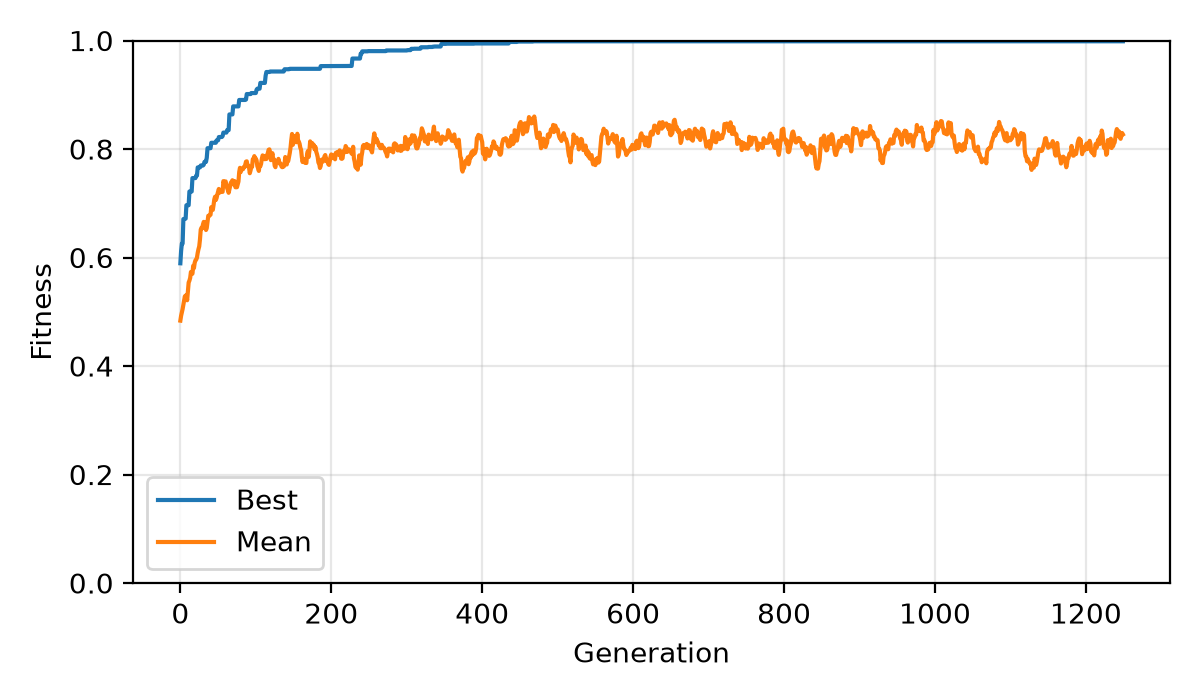
\includegraphics[width=\linewidth]{figures/fitness.png}
  \caption{Best and mean fitness per generation for the default configuration
    (mutation rate 0.05, seed 1).}
  \label{fig:fitness}
\end{figure}

\begin{figure}
  \centering
  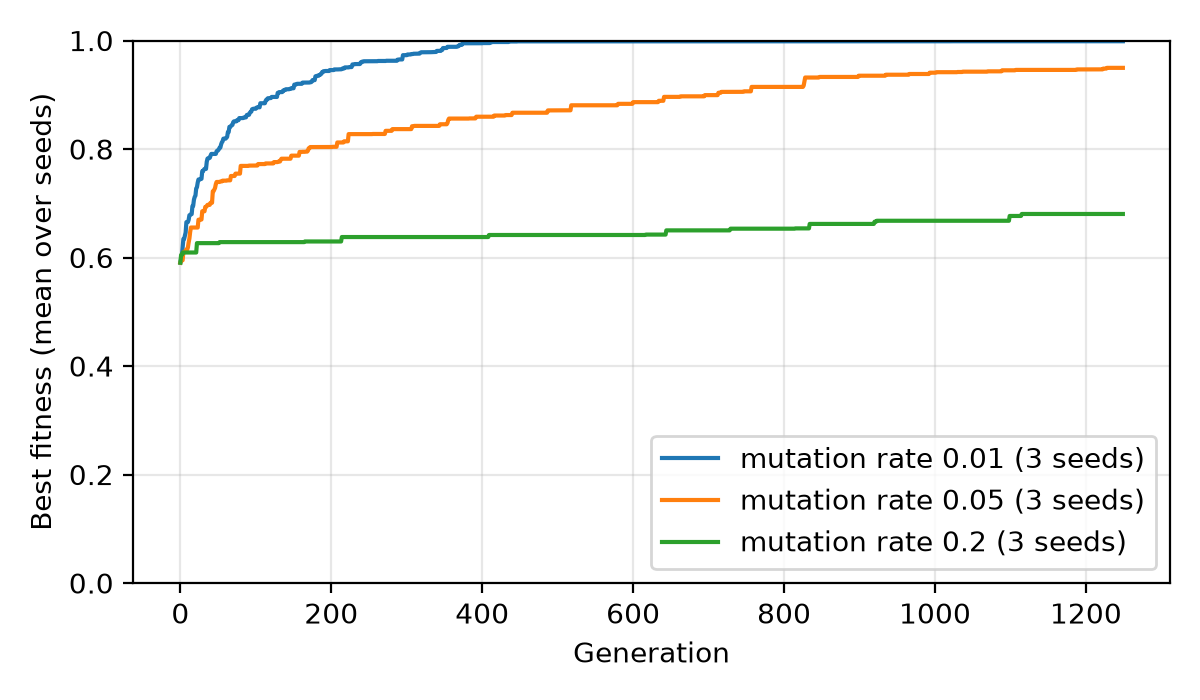
\includegraphics[width=\linewidth]{figures/comparison.png}
  \caption{Best fitness per generation for each mutation rate, averaged over 3 seeds.}
  \label{fig:comparison}
\end{figure}

\begin{table}
  \centering
  \begin{tabular}{lcccc}
    \toprule
    Rate & Seed 1 & Seed 2 & Seed 3 & Mean \\
    \midrule
    0.01 & 0.999 & 0.999 & 0.999 & 0.82 \\
    0.05 & 0.957 & 0.986 & 0.906 & 0.58 \\
    0.2  & 0.704 & 0.644 & 0.693 & 0.39 \\
    \bottomrule
  \end{tabular}
  \caption{Best fitness at the last generation (1249) per mutation rate and seed, and
    population mean fitness
    averaged over the 3 seeds.}
  \label{tab:results}
\end{table}


\nocite{*}
\bibliography{references}

\end{document}
